\chapter{Basic usage}

The ESTER code calculates the axisymmetric structure and mean flows
of an isolated (non-magnetic) rotating star. It uses realistic physics
(tabulated opacities and EOS like those of OPAL) and completely
accounts for the deformation of the star.  The mean flows are calculated
self-consistently in the limit of low viscosity, so there is no need
to impose an arbitrary prescription for the differential rotation of
the star.  Surface convection is not included yet, so the computations
are limited to early-type stars, that is to stars with mass typically
above $\sim 2 M_\odot$.

Presently, chemical evolution is not included, but it can be faked
by tweaking the fractional abundance of hydrogen in the convective core.

For a detailed description of the physics involved
in the models, see Rieutord \& Espinosa Lara 2013
(\href{http://arxiv.org/abs/1208.4926}{arXiv:1208.4926},
LNP 865, p.49), Espinosa Lara \& Rieutord 2013
(\href{http://arxiv.org/abs/1212.0778}{arXiv:1212.0778},
in A\&A 552, A35) and Rieutord et al. 2016
(\href{http://userpages.irap.omp.eu/~mrieutord/articles/2016JCP.pdf}),
in J. Comp. Phys. vol.  318, 277-304.  The code is still in development,
so new functionality will be added in future versions.

To execute the program, use the following syntax:
\begin{shell}
    $ ester command [options]
    !$
\end{shell}
where \texttt{command} can be:
\begin{description}
    \item[{\tt 1d}]: Calculate the structure of a 1D non-rotating star
    \item[{\tt 2d}]: Calculate the structure of a 2D rotating star
    \item[{\tt output}]: Generate a custom output file
    \item[{\tt info}]: Get information about a model file
    \item[{\tt help}]: Get help
\end{description}

\section{Configuration files}

The main configuration file is located at
\texttt{\$prefix/share/ester/config/star.cfg}.
This file contains the main options for the program, which are

\begin{itemize}
\item {\tt maxit} (default 200).
Maximum number of iterations. After {\tt maxit} iterations, the program
exits normally and the output file is saved, even if it has not completely converged.
\item {\tt minit} (default 1).
Minimum number of iterations. It may occur that the value of the error
for the first iteration is not representative. With this parameter we force the solver to
do at least {\tt minit} iterations. This parameter is superseded by {\tt maxit}, for example
if {\tt maxit=5} and {\tt minit=10}, the solver will do only 5 iterations.
\item {\tt tol} (default 1e-8). 
The relative tolerance for checking the convergence of the model.
\item {\tt newton\_dmax} (default 0.5).
After one step of the Newton's method, the maximum relative change
allowed for a variable is given by {\tt newton\_dmax}. If necessary the iteration is relaxed
by a parameter $h$
$$\vec x^{N+1}=\vec x^N+h \delta\vec x^N$$
according to this value.
This parameter can be used to stabilize the convergence when the initial estimation is far
from the solution.
\item {\tt output\_file} (default {\tt star.out}). Name of the output file.
\item {\tt output\_mode} (default {\tt b}). Type of the output file {\tt b} for binary
and {\tt t} for text output.
\item {\tt verbose} (default 1). Level of verbosity, from 0 (quiet) to 4.
%\item {\tt plot\_device} (default {\tt /XSERVE}. Plotting device for PGPLOT, 
%see the documentation of PGPLOT for details. For output in a X window use {\tt /XSERVE}.
%To disable the graphic output use {\tt /NULL}.
%\item {\tt plot\_interval} (default 10). Minimum time in seconds to update the graphic output.
\end{itemize}

All these options can be specified in the file 
\texttt{\$prefix/share/ester/config/star.cfg} in the form {\tt
option\_name=option\_value} (one per line) and in the command line as {\tt
-option\_name option\_value}.
The options specified in the command line have precedence over those specified
in the configuration file.

\bigskip
There are some additional options that can be included in the command line:

\begin{itemize}
\item[] {\tt -input\_file} {\it infile}. Use the file {\it infile} as the starting point
for the iteration.
\item[] {\tt -i} {\it infile}. Same as {\tt -input\_file} {\it infile}.
\item[] {\tt -o} {\it outfile}. Same as {\tt -output\_file} {\it outfile}.
\item[] {\tt -param\_file} {\it file}. Where {\it file} contains the parameters of the 
stellar model to be calculated (see below).
\item[] {\tt -p} {\it file}. Same as {\tt -param\_file} {\it file}.
\item[] {\tt -ascii}. Same as {\tt -output\_mode t}.
\item[] {\tt -binary}. Same as {\tt -output\_mode b}.
\item[] {\tt -noplot}. disable runtime plotting %Same as {\tt -plot\_device /NULL}.
\item[] {\tt -v}{\it n}. Same as {\tt -verbose} {\it n}.
\end{itemize}

\section{Default values}

Default values to be used by {\tt star1d} or {\tt star2d} may be set up
with the files 
\begin{itemize}
\item[-]{\tt \$prefix/share/ester/config/1d\_default.par} 
\item[-]{\tt \$prefix/share/ester/config/2d\_default.par}.
\end{itemize}

In the distribution of ESTER, the proposed default values are such that
the star is divided in 8 domains with 30 points in each domains. Opacities
and equation of state are computed through OPAL tables. These inputs
allow the calculation of a 1D 3 M$_\odot$ model (but not only of course)
from scratch. 2D-models cannot be computed from scratch and need a first
1D model to start with.

\subsection{Chemical composition}

The default chemical composition is the solar mixture of
\cite{GN93} as given in tables GN93hz. Presently (nov. 2017), it cannot be
changed (easily!).

\section{{\tt ester 1d} input parameters}

The input parameters for {\tt ester 1d} can be passed in the command line
or in a text file specified with the option {\tt -param\_file} {\it file}
(or just {\tt -p} {\it file}). It can also be used simultaneously, in
this case the parameters given in the command line take precedence over
those specified in the file. In the text file they are written in the
form {\tt param\_name}={\it param\_value} and in the command line as {\tt
-param\_name} {\it param\_value}.  Here is the list of valid parameters

\begin{itemize}
\item {\tt ndomains}. The number of subdomains to use.
\item {\tt npts}. Number of points in each subdomain. It is specified as a 
comma-separated list. 
If only one value is specified, it will be used for all the subdomains, for example:
\mint{bash}|$ star1d -ndomains 4 -npts 20,20,20,20|  %$
is equivalent to
\mint{bash}|$ star1d -ndomains 4 -npts 20|  %$

\item {\tt M}. The mass in units of solar mass.
\item {\tt X}. Mass fraction of hydrogen.
\item {\tt Z}. Mass fraction of metals.
\item {\tt Xc}. Fraction of the hydrogen abundance present in the convective core. The profile
of hydrogen abundance will be in the form
$$X(\vec r)=\left\{
\begin{array}{ll}
\mathtt{X}\times \mathtt{Xc}&\mbox{if $\vec r$ is in the convective core}\\
\mathtt{X}&\mbox{otherwise}
\end{array}\right.$$
If there is no convective core, this parameter is ignored.

\item {\tt surff}. This parameter is used for truncating the stellar model
at some point below the surface. The surface pressure will be {\tt surff}
times the "real´´ value and the boundary conditions will be adjusted
correspondingly. This parameter is provided only for testing purposes as
it does not produce an accurate representation of the internal layers
of the star. For regular calculations it should be {\tt surff=1}.

\item {\tt Tc}. Initial estimation of the central temperature. To be
updated during the calculation.

\item {\tt pc}. Initial estimation of the central pressure. To be updated during the
calculation.
\item {\tt opa}. Type of opacity law. Possible values are:
\begin{itemize}
\item {\tt opal}. OPAL opacities from \cite{GN93}.
\item {\tt houdek}. Houdek's interpolation of OPAL opacities (smoother),
see Houdek and Rogl (1996), "On the accuracy of opacity interpolation
schemes", {\it Bull. Ast. Soc. India}, {\bf 24}, 317.
\item {\tt kramer}. Kramer's opacity.
\end{itemize}
\item {\tt eos}. Type of equation of state. Possible values are:
\begin{itemize}
\item {\tt opal}. OPAL equation of state.
\item {\tt ideal}. Ideal gas.
\item {\tt ideal+rad}. Ideal gas with radiation.
\end{itemize}
\item {\tt nuc}. Type of nuclear reactions. Possible values are:
\begin{itemize}
\item {\tt simple}. Simplified formulation of pp and CNO cycles. 
\item {\tt cesam}. NACRE reaction rates as implemented in the ppcno9 chain of the CESAM code.
\end{itemize}
\item {\tt atm}. Type of atmosphere. At the moment, only {\tt simple} is implemented.
\item {\tt core\_convec} (default 1). Use 0 to disable core convection.
\item {\tt min\_core\_size} (default 0.01). The minimum size of the convective core
in fraction of the polar radius).
\end{itemize}
If some parameters are omitted, the program will take the value from the input file (set with
{\tt -input\_file} or {\tt -i}) or from the default parameters file in 
{\tt ester/config/1d\_default.par} when no input file is specified.

\bigskip
\noindent {\bf Note on chemical composition:} In the programme a set of
ratios is proposed in the file physics/composition.cpp, namely

\begin{center}

\begin{tabular}{c|l}
\hline
	   &   \\
	Element & Mass fraction \\
	   &   \\
        H  & X \\
        He3  & 3.15247417638132e-04*(1.-X-Z) \\
        He4  & (1.-X-Z)-X(He3) \\
        C12  & Z*1.71243418737847e-01 \\
        C13  & Z*2.06388003380057e-03 \\
        N14  & Z*5.29501630871695e-02 \\
        N15  & Z*2.08372414940812e-04 \\
        O16  & Z*4.82006487350336e-01 \\
        O17  & Z*1.95126448826986e-04 \\
	   &   \\
\hline
\end{tabular}

\end{center}

These ratios of the mass fraction of some elements are used only with
the option -nuc cesam. They correspond (approximately) to the chemical
abundances of \cite{GS98}



\section{{\tt ester 2d} input parameters}

{\tt ester 2d} needs a non-rotating 1D model
calculated with {\tt ester 1d} or a previous 2D-model.

The program {\tt ester 2d} admits the same parameters than {\tt ester 1d}
plus some extra specific options:

\begin{itemize}
\item {\tt nth}. The number of grid points in latitude.
\item {\tt nex}. Number of radial points in the external domain.
\item {\tt Omega\_bk}. Angular velocity at the equator in units of the critical velocity
$\Omega_c=\sqrt{\frac{GM}{R_e^3}}$.
\item {\tt Ekman}. Ekman number (gives the amplitude of the meridional circulation).
\end{itemize}

\section{{\tt ester evol} input parameters}

At the moment {\tt ester evol} is the poor man recipe for stellar
evolution of intermediate mass stars. It assumes that the convective core
is the only part of the star that burns hydrogen. It also assumes that
the star evolves at constant angular momentum. This latter assumption
is therefore inappropriate for massive stars that are known to lose a
lot of mass. It should be fine for stars with masses less than say 8\msun.

From a ZAMS model, Xc is set to 1 (same hydrogen content in the core and in
the envelope). Usage is 

\begin{minted}{bash}
$ ester evol -dXc 0.01 -i M4_04 -o M4_04_evol
\end{minted}

\noindent where  dXc gives the variation of Xc from one step to the next. Output
files are numbered {\tt M4\_04\_evol\_0000, M4\_04\_evol\_0001,..} Note
that the output files give an evolution but not a time-evolution since
the nuclear clock is not installed.

Note that {\tt dXc} may also be negative so as to permit an evolution
backward in time.





\section{Some recipes}

The typical workflow to calculate a model starts with the calculation of
the corresponding 1D model and using it as an input for {\tt star2d}. For
example, to calculate the structure of a 5$M_\odot$ star with OPAL
opacity rotating at with $\Omega=0.5\Omega_c$ we can do:

\begin{minted}{bash}
$ ester 1d -M 5 -opa opal -o model1d
$ ester 2d -i model1d -nth 24 -Omega_bk 0.5 -o model2d
\end{minted}

As the code uses the Newton's method, it is not possible
to converge to a solution if the initial estimation is too far from
it. In this case we can use some intermediate steps.  For example, if
we want to calculate the structure of a 2.5$M_\odot$ star rotating with
$\Omega=0.9\Omega_c$, we can do

\medskip
\noindent\begin{tabular}{lp{4.5cm}}
\verb|$ ester 1d -M 2.5 -o model1d |  
&(Start with a non rotating 1D model)\\
\verb|$ ester 2d -i model1d -nth 24 -Omega_bk 0.5 -o model2d| &	
(Using an intermediate value for rotation) \\
\verb|$ ester 2d -i model2d -nth 32 -Omega_bk 0.9 -o model2d| &	
(Calculating the final model) 
\end{tabular}
\medskip

Executing {\tt ester 2d} with {\tt maxit=0} can be used to interpolate a
model without recalculating it, like

\medskip
\noindent
\verb|$ ester 2d -i model -npts |{\it npts\_new}\verb| -nth |{\it nth\_new}\verb| -o model_interp -maxit 0|

\medskip
Pressing Ctrl-C at any time during the execution of {\tt ester 2d} will
terminate the program, giving the possibility of finishing the current
iteration and write the result in the output file.

\section{Spatial resolution and memory requirements}

The ESTER code uses a direct method to solve the equations of structure
of a star. This type of method involves the factorization of a big matrix
that arises from the discretization of the equations.  The main drawback
is that memory requirements are high, but the stiffness of the equations
prevents the convergence of an iterative (matrix-free) method that would
be more memory efficient.

The memory needed by the calculation can be estimated as:

$$\mathrm{RAM\ Used}\gtrsim25\times n_d\times n_r^2 \times n_\theta^2 \times 8\, \mathrm{bytes}$$

where

\medskip

\begin{tabular}{l}
$n_d$: Number of domains \\
$n_r$: Number of ``radial" points per domain \\
$n_\theta$: Number of points in latitude \\
\end{tabular}

\medskip

Of course, this is a lower limit, the actual memory used can be between
$\sim$10\% and $\sim$50\% higher than this value.  This overhead
increases with the number of domains and decreases with the overall
number of points. As an example, the following table shows the memory
usage for some configurations (this is only approximated, real values
are machine-dependent):

\begin{center}
\begin{tabular}{c|c|c|c|c|c}
$n_d$&$n_r$&$n_\theta$&RAM (estimated)&RAM (real)&Overhead\\
\hline
8&30&24& 791 Mb & 986 Mb & 25\% \\
8&50&32& 3.81 Gb & 4.27 Gb & 12\% \\
32&25&32& 3.81 Gb & 4.61 Gb & 21\% \\
\end{tabular}
\end{center}

The first case correspond to the default values and, in most cases,
gives a decent representation of the structure of the star for moderate
rotation rates.  If more precision is required, we need to increase the
resolution. In particular, to achieve a good precision for high rotation
values, the number of points in latitude should be incremented.

As seen in the second and third cases in the table, the total number
of radial points $n_d\times n_r$ can be increased, without affecting
considerably the memory usage, just by increasing the number of domains.
Or equivalently, we can reduce the memory requirements by distributing
the radial points over more domains.

As a rule of thumb, if the number of domains is doubled, keeping the
total number of radial points, the memory required is reduced in a factor
$\sqrt{2}$. However this does not necessarily imply an improvement
in precision, as the order of the integration method is also reduced,
so it should be used carefully.

\subsection{Estimating the precision of the output model}

The ESTER code uses spectral methods to calculate the structure of
the star.  The star is subdivided in a certain number of domains and, in
each domain, the variables are represented by a double truncated series
of orthogonal polynomials in the ``radial" ($\zeta$) and ``horizontal"
$\theta$ directions, for instance

\[\rho(\zeta,\theta)=
\sum_{i=0}^{n_r-1}\sum_{j=0}^{n_\theta-1}\rho_{ij}T_i(\zeta)P_j(\cos\theta)\]
where $T_i$ and $P_j$ are Chebyshev and Legendre polynomial
respectively.
When $n_r$ and $n_\theta$ are high enough, the spectral representation
converges to the exact function.  To check the convergence of
the solution $\rho_{ij}$, the corresponding normalised spectra for
the density ($\rho$) are shown in the graphics output of ESTER (see
\ref{fig:spectrum1d} and \ref{fig:spectrum2d}).

\begin{figure}[H]
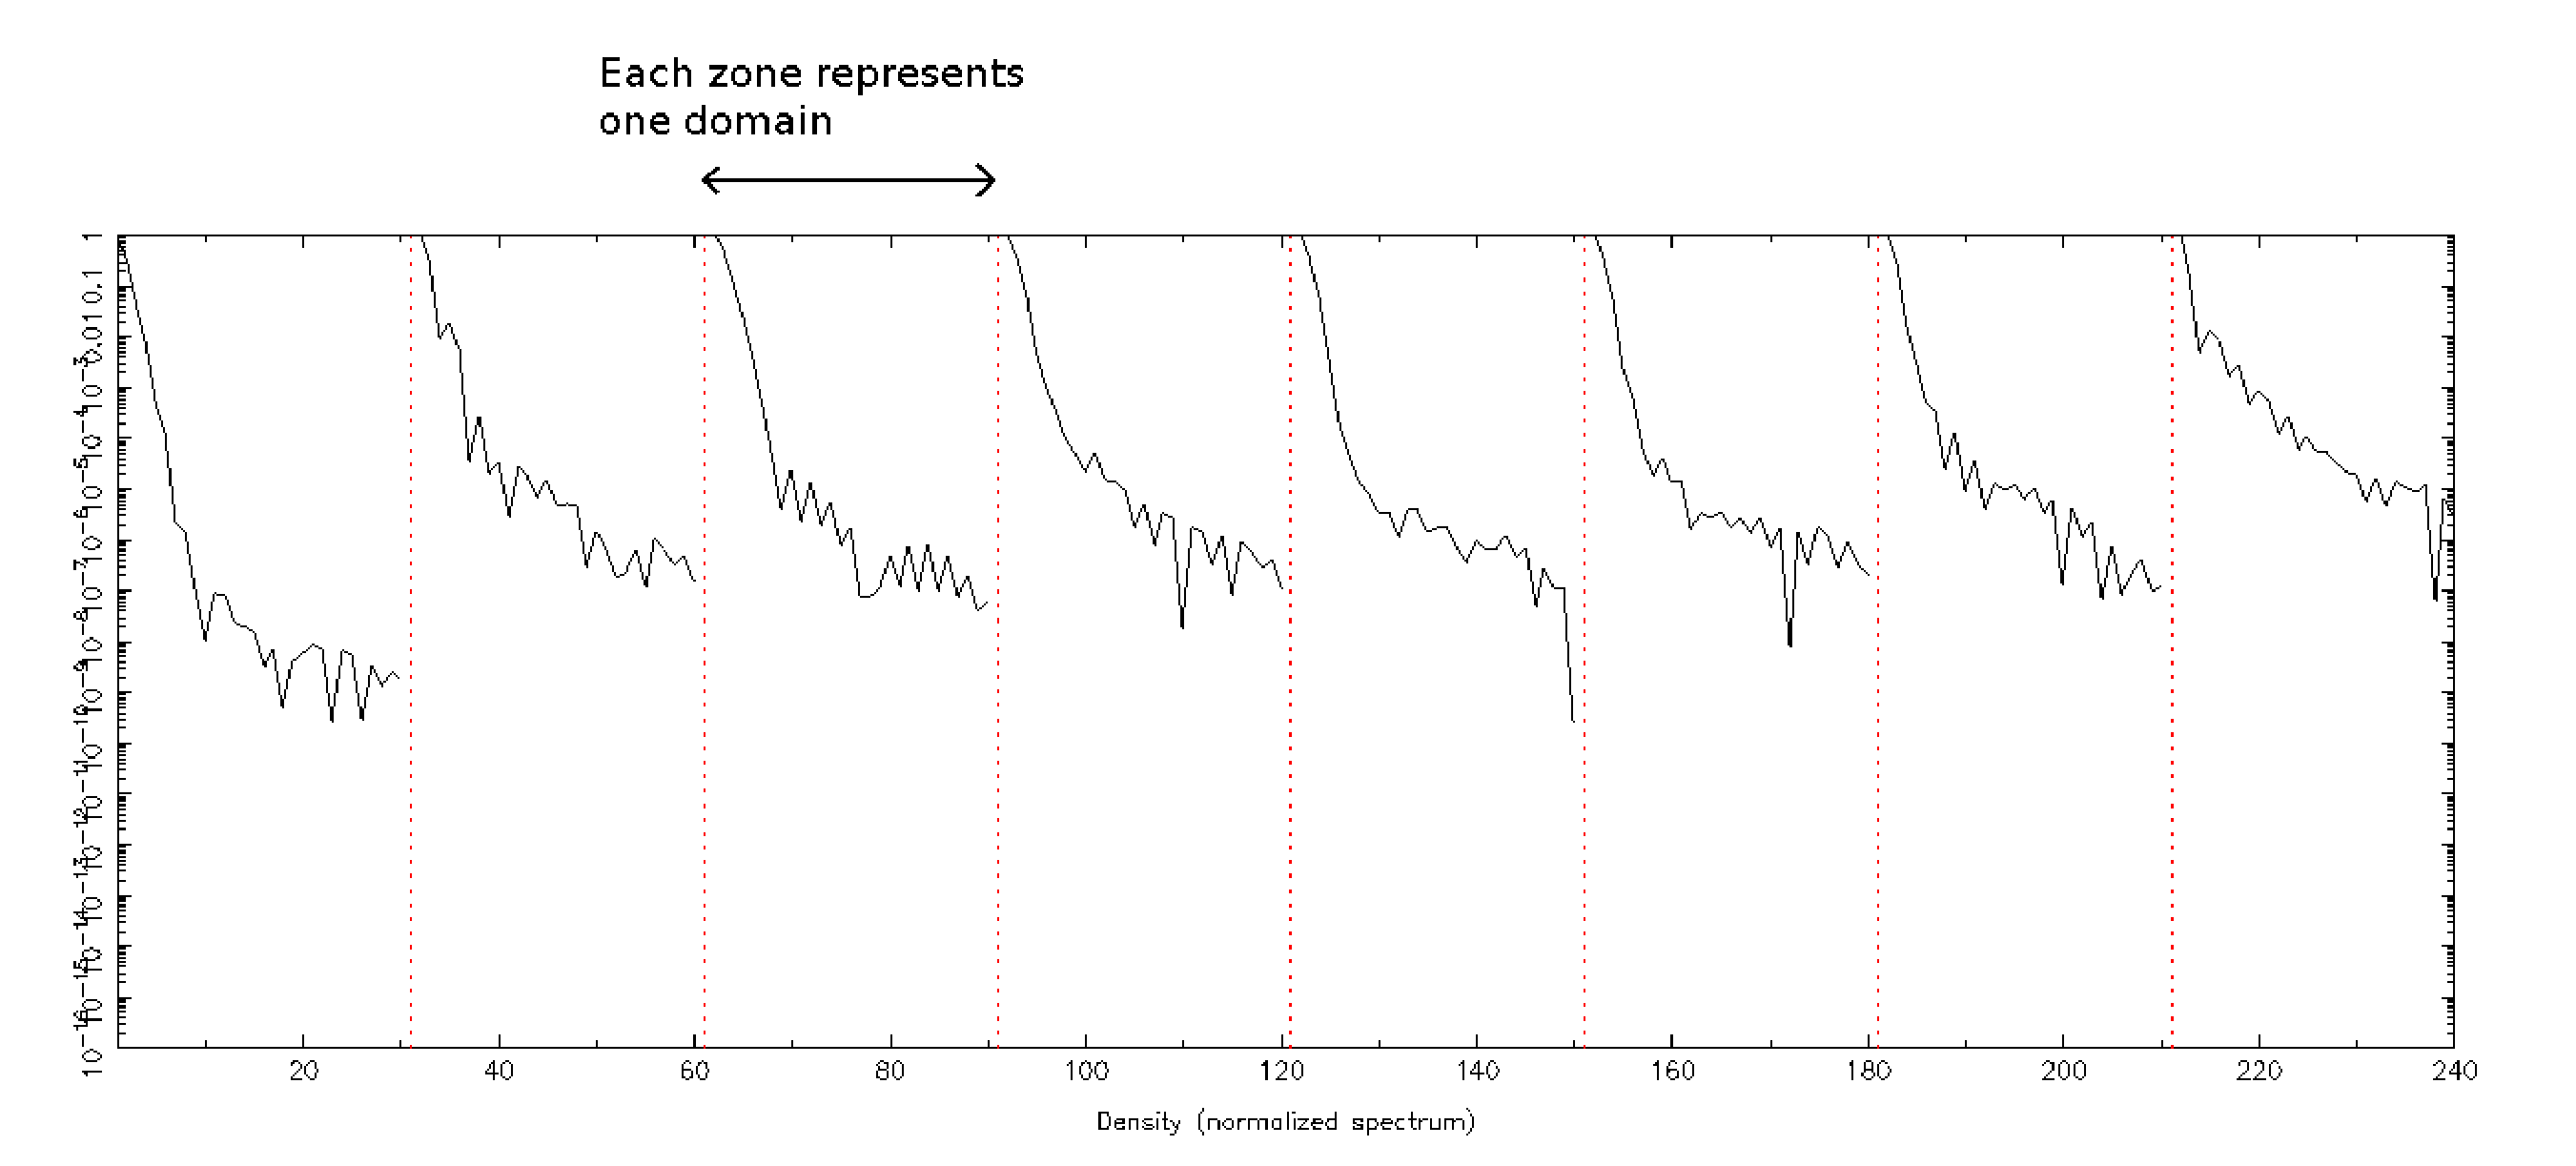
\includegraphics[width=\textwidth]{fig/spectrum1d.eps}
\caption{Example of spectrum plot showing the normalised coefficients $\rho_{i}$ in a logarithmic scale
 in the graphical output of {\tt ester 1d}.
\label{fig:spectrum1d}}
\end{figure} 
\begin{figure}[H]
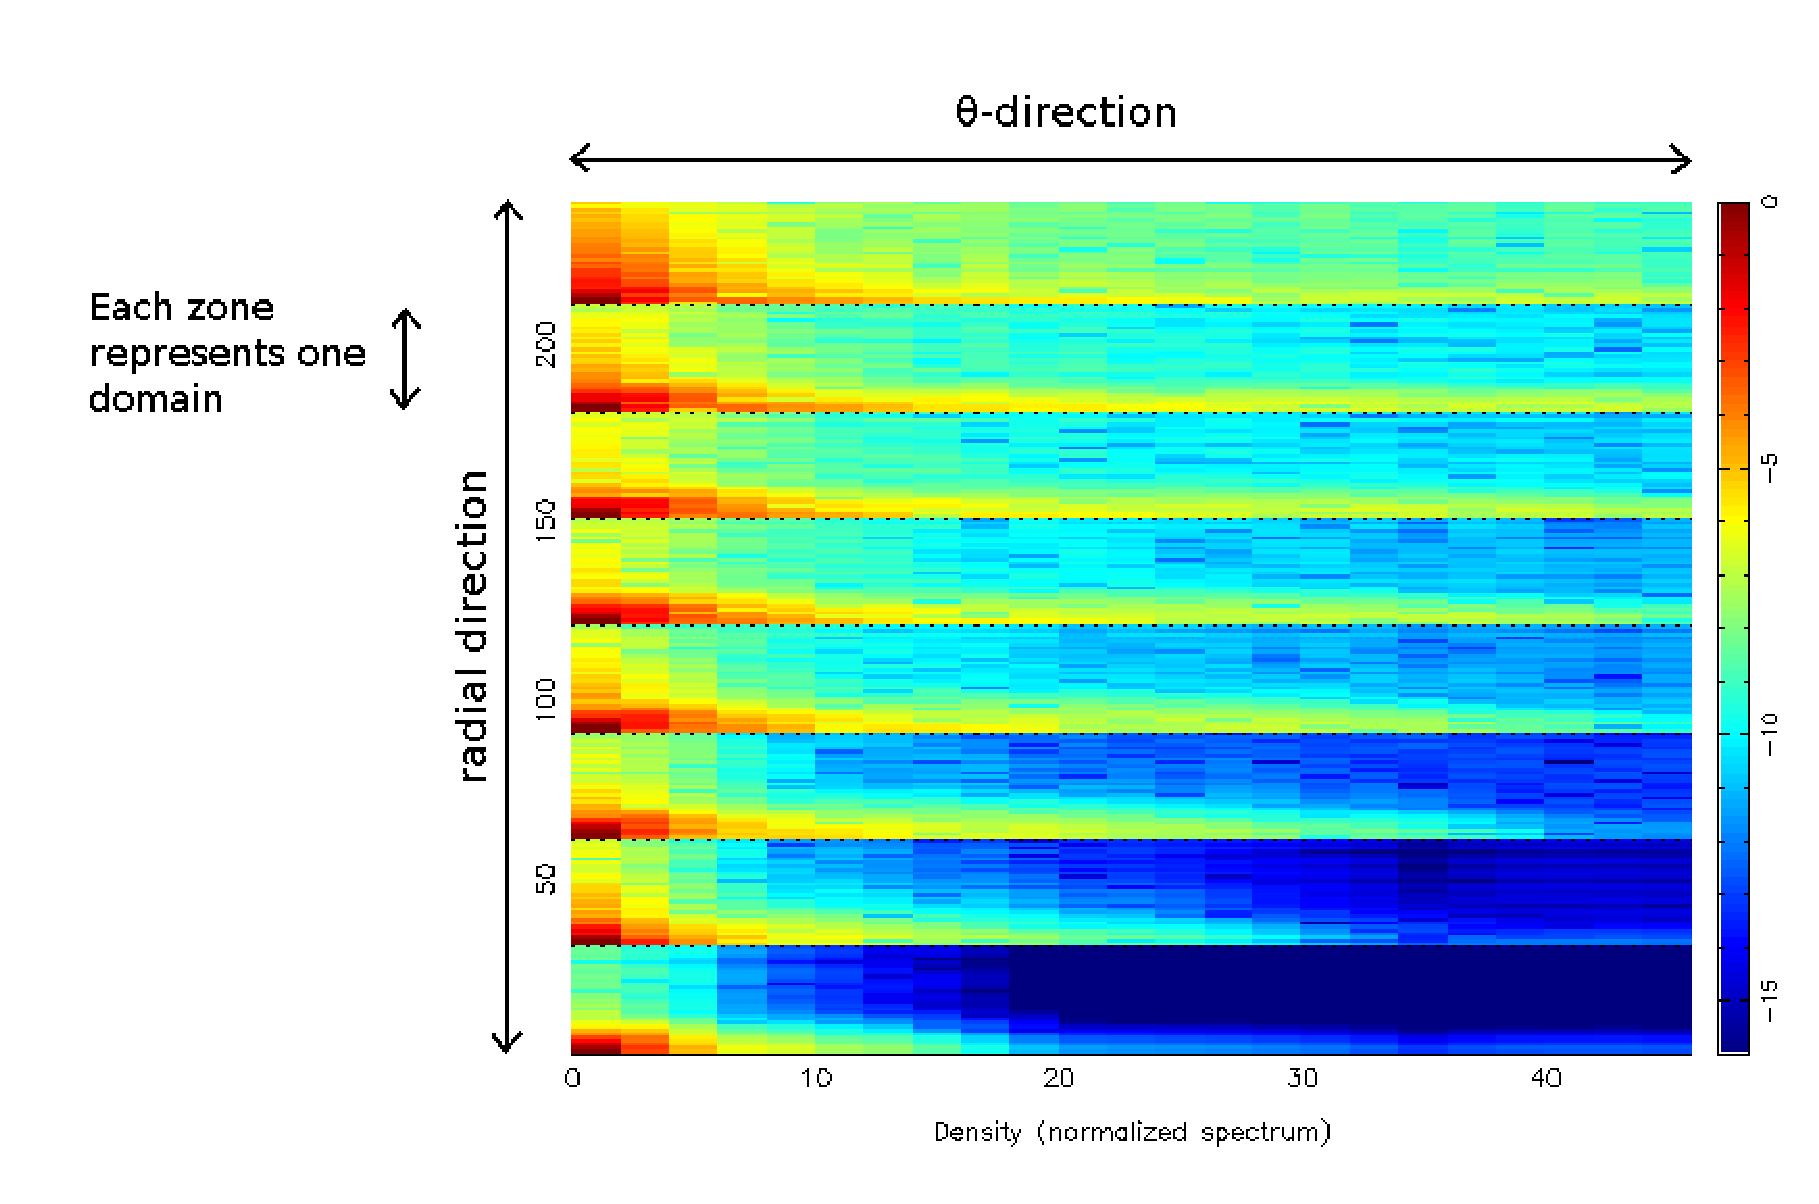
\includegraphics[width=\textwidth]{fig/spectrum2d.eps}
\caption{Example of 2D-spectrum showing the logarithm of the normalised coefficients $\rho_{ij}$ 
in the graphical output of {\tt ester 2d}.
\label{fig:spectrum2d}}
\end{figure}

There are two other indicators that can be used to estimate the quality
of the solution:

\begin{itemize}
\item {\bf The virial test}. It is the normalised residual resulting from
the virial theorem.  Ideally, it should be zero. It is mainly influenced
by the internal layers and even with low resolution we can get very good
values $\lesssim10^{-9}$.

\item {\bf The energy test}. It is the relative difference between
the luminosity of the star obtained as the integral over the volume
of the energy generation rate and that obtained as the integral of the
energy flux at the surface. It is highly influenced by the quality of
the solution in the most external layers. Due to the use of tabulated
opacities which are not quite smooth, the energy test will be always
higher than $10^{-5}$--$10^{-6}$.

\end{itemize}

In the following table, we can see examples of the precision achieved for
three different configurations. The three configurations use approximately
1 Gb of RAM, but have different number of domains. We have used a model
with 1600 radial points distributed over 16 domains and $n_\theta=48$
(approx. 70 Gb of RAM) as a reference to calculate the errors.

\begin{center}
\begin{tabular}{c|c|c||c|c|c|c|c|c}
$n_d$ & $n_r$ & $n_\theta$ & Virial test & Energy test &
$\Delta\rho/\rho$ & $\Delta R/R$ & $\Delta T_\mathrm{eff}/T_\mathrm{eff}$ & $\Delta \Omega/\Omega$ \\
\hline
8 & 30 & 24 & 1.848e-09 & 1.192e-03 & 
1.613e-04 & 5.157e-05 & 3.338e-04 & 3.739e-04 \\
16 & 21 & 24 & 1.851e-11 & 1.726e-04 &
1.065e-04 & 4.702e-05 & 1.215e-04 & 4.446e-04 \\
32 & 15 & 24 & 3.377e-10 & 3.447e-05 &
2.780e-05 & 2.021e-06 & 1.736e-05 & 3.095e-04 \\
\end{tabular}
\end{center}

\section{Generating custom output files}

The output files generated by {\tt ester 1d} and {\tt ester 2d} contain
just the minimal information necessary to reconstruct the model. However,
sometimes a more detailed output is required.  This can be done using
{\tt ester output}. This program reads a template from the standard input
and write the result in the standard output.  A typical call would be

\medskip
\noindent
\verb|$ ester output |{\it model\_file}\verb| < |{\it template\_file}\verb| > |{\it output\_file}

\medskip

The template file is a regular text file with the following rules:

\begin{itemize}
\item Plain text is copied from the template to the output file. It
cannot contain the reserved characters {\tt \$} and {\tt \textbackslash}.

\item Line breaks are ignored. To insert a line break in the output file
you have to insert a blank line in the template.

\item Variables from the model are written in the form \mbox{{\tt
\$\{}{\it var}{\tt ,}{\it fmt}{\tt \}}}, where {\it var} is the code
for the variable (see table below) and {\it fmt} is a valid format for
the C function {\it printf} (e.g. {\tt \%d} for an integer, {\tt \%f}
for float, {\tt \%e} for exponential notation).  If {\tt fmt} is omitted
{\tt\$\{}{\it var}{\tt \}} the variable is written in binary format.

\end{itemize}

\begin{longtable}{|l|p{8cm}|c|c|}
\caption{Non-exhaustive list of variables codes for the model in the template
file. Dimensional quantities are in cgs}\\
\hline
\bf Code&\bf Description&\bf star1d&\bf star2d\\
\hline\hline
nr&\# of radial points&*&*\\
\hline
nth&\# of points in latitude&&*\\
\hline
ndomains&\# of domains&*&*\\
\hline
npts&\# of radial points in each domain&*&*\\
\hline
xif&Position of each domain&*&*\\
\hline
nex&\# of radial points in the external domain&&*\\
\hline
surff&Parameter surff (see above)&*&*\\
\hline
conv&\# of convective domains&*&*\\
\hline
Omega&Angular velocity at the equator in $\sqrt{\frac{P_c}{\rho_cR^2}}$&&*\\
\hline
Omegac&Critical angular velocity $\Omega_c=\sqrt{\frac{GM}{R_e^3}}$ in $\sqrt{\frac{P_c}{\rho_cR^2}}$&&*\\
\hline
Omega\_bk& $\Omega/\Omega_c$   &&*\\
\hline
X&Hydrogen initial abundance&*&*\\
\hline
Z&Metal abundance&*&*\\
\hline
Xc&Fraction of X in the convective core&*&*\\
\hline
rhoc&Central density (g/cm$^3$)&*&*\\
\hline
Tc&Central temperature (K)&*&*\\
\hline
pc&Central pressure (cgs)&*&*\\
\hline
M&Mass (grams)&*&*\\
\hline
R&(Polar) Radius (cm)&*&*\\
\hline
Rp&Polar radius (cm)&&*\\
\hline
Re&Equatorial radius (cm)&&*\\
\hline
L&Luminosity (erg/s)&*&*\\
\hline
M/M\_SUN&Mass in solar units&*&*\\
\hline
R/R\_SUN&(Polar) Radius in solar units&*&*\\
\hline
Rp/R\_SUN&Polar radius in solar units&&*\\
\hline
Re/R\_SUN&Equatorial radius in solar units&&*\\
\hline
L/L\_SUN&Luminosity in solar units&*&*\\
\hline
r&Radius (non-dimensional) &*&*\\
\hline
rt& $\partial_\theta r$ (non-dimensional) &*&*\\
\hline
rz& $\partial_\zeta r$ (non-dimensional) &*&*\\
\hline
rzt& $\partial_{\zeta\theta} r$ (non-dimensional) &*&*\\
\hline
rzz& $\partial_{\zeta\zeta} r$ (non-dimensional) &*&*\\
\hline
gzz& $g_{\zeta\zeta}$ (non-dimensional) &*&*\\
\hline
gzt& $g_{\zeta\theta}$ (non-dimensional) &*&*\\
\hline
z&Radial variable (non-dimensional)&*&*\\
\hline
th&Colatitude (rd) (2D grid) &&*\\
\hline
rex&External radius&&*\\
\hline
phi&Gravitational potential&*&*\\
\hline
phiex&Gravitational potential of the external domain&&*\\
\hline
rho&Density (non-dimensional)&*&*\\
\hline
p&Pressure (non-dimensional)&*&*\\
\hline
T&Temperature (non-dimensional)&*&*\\
\hline
w&Angular velocity in $\sqrt{\frac{P_c}{\rho_cR^2}}$&&*\\
\hline
G&Stream function for the meridional circulation&&*\\
\hline
Xr&Hydrogen abundance $X(r,\theta)$ not in use (yet) &*&*\\
\hline
N2&Squared Brunt-V\"ais\"al\"a frequency (in rd$^2$/s$^2$)&*&*\\
\hline
opa&Type of opacity&*&*\\
\hline
opa.k&Rosseland mean opacity (cm$^2$/g) &*&*\\
\hline
opa.xi&Thermal conductivity ($\chi$)&*&*\\
\hline
opa.dlnxi\_lnT&$\left(\frac{\partial\log\chi}{\partial\log T}\right)_{\rho,\mu}$&*&*\\
\hline
opa.dlnxi\_lnrho&$\left(\frac{\partial\log\chi}{\partial\log\rho}\right)_{T,\mu}$&*&*\\
\hline
eos&Type of equation of state&*&*\\
\hline
eos.G1&$\Gamma_1$&*&*\\
\hline
eos.cp&$c_p$ (cgs) &*&*\\
\hline
eos.del\_ad&$\nabla_{ad}$&*&*\\
\hline
eos.G3\_1&$\Gamma_3-1$&*&*\\
\hline
eos.cv&$c_v$ (cgs)&*&*\\
\hline
eos.prad&Radiation pressure&*&*\\
\hline
eos.chi\_T&$\chi_T=\left(\frac{\partial\log p}{\partial\log T}\right)_{\rho,\mu}$&*&*\\
\hline
eos.chi\_rho&$\chi_\rho=\left(\frac{\partial\log p}{\partial\log\rho}\right)_{T,\mu}$&*&*\\
\hline
eos.d&$d=\frac{\chi_T}{\chi_\rho}=-\left(\frac{\partial\log\rho}{\partial\log T}\right)_{p,\mu}$&*&*\\
\hline
nuc.eps&Energy generation rate per unit mass (cgs)&*&*\\
\hline
nuc.pp&Energy generation rate per unit mass (pp-chain)&*&*\\
\hline
nuc.cno&Energy generation rate per unit mass (CNO cycle)&*&*\\
\hline
Teff&Surface effective temperature $T_\mathrm{eff}(\theta)$ (Kelvin) &*&*\\
\hline
gsup&Surface effective gravity surface $g_\mathrm{eff}(\theta)$ (cm/s$^2$) &*&*\\
\hline
D&Radial differentiation matrix $\frac{\partial}{\partial\zeta}$ for 2D models,
$\frac{\mathrm{d}}{\mathrm{d}r}$ for 1D models&*&*\\
\hline
I&Radial integration matrix&*&*\\
\hline
Dex&Radial differentiation matrix for the external domain&&*\\
\hline
Dt&Angular differentiation matrix $\frac{\partial}{\partial\theta}$ for symmetric variables&&*\\
\hline
Dtodd&Angular differentiation matrix for antisymmetric variables&&*\\
\hline
Dt2&Second order angular differentiation matrix for symmetric variables&&*\\
\hline
It&Angular integration matrix over $\mu=\cos\theta$ &&*\\
\hline
\end{longtable}
For 2D variables, their values at the collocation points are written
in the output file in matrix form. Each line corresponds to a different
value of the colatitude $\theta$ {\em starting
at the equator.} Namely, if {\tt nth=8}, we have

\beqa
\theta_0&=&1.47564028,\; \theta_1=1.28533144,\; \theta_2=1.0950334,\;
\theta_3=0.90475753,\; \theta_4=0.71452525,\\
\theta_5&=&0.52438664,\; \theta_6=0.33449864,\; \theta_7=0.14572468
\eeqa
while the values of a field are ordered as

$$\begin{array}{cccc}
p(\zeta_0,\theta_0)&p(\zeta_1,\theta_0)&p(\zeta_2,\theta_0)&\cdots\\
p(\zeta_0,\theta_1)&p(\zeta_1,\theta_1)&p(\zeta_2,\theta_1)&\cdots\\
p(\zeta_0,\theta_2)&p(\zeta_1,\theta_2)&p(\zeta_2,\theta_2)&\cdots\\
\vdots&\vdots&\vdots&
\end{array}$$
$\zeta$ being the radial spheroidal coordinate.  Similarly, 1D variables
can be seen as a column vector and are written in one line in the output
file, terminated by a new line character.  This behavior can be inverted
by writing this line in the template file

\begin{verbatim}
\conf{transpose=1}
\end{verbatim}
After this command, the variables will be written row wise, i.e. one line
for each value of the radial coordinate. Note that it does not affect
variables written in binary format, which are always column wise. To
recover the original behaviour we use

\begin{verbatim}
\conf{transpose=0}
\end{verbatim}
The original grid  does not contain points at the equator nor at the pole. If
we want the values at these points we should write

\begin{verbatim}
\conf{equator=1}
\conf{pole=1}
\end{verbatim}
By default, the output uses cgs units. If we want the normalized values
used internally by the code, we simply put

\begin{verbatim}
\conf{dim=0}
\end{verbatim}
These control commands can be written anywhere in the template file,
in separated lines, affecting only the code that appears below them.

Let's see an example.

Template file:
\begin{minted}[frame=single]{text}
Model of ${M/M_SUN,%.2f} solar masses and R=${R,%e} cm

rotating with Omega=${Omega_bk,%f} Omegac

${nr,%d} radial points and 
${nth,%d} latitudinal points

\conf{pole=1}
\conf{equator=1}
r:

${r,%e}
Pressure:

${p,%.14e}

\end{minted} 
%$

Output file:
\begin{minted}[frame=single]{text}
Model of 2.50 solar masses and R=1.219822e+11 cm
rotating with Omega=0.900000 Omegac
240 radial points and 32 latitudinal points
r:
0.000000e+00 4.944313e+07 1.971944e+08 4.415355e+08 7.796539e+08 ...
0.000000e+00 4.944313e+07 1.971944e+08 4.415355e+08 7.796539e+08 ...
0.000000e+00 4.944313e+07 1.971944e+08 4.415354e+08 7.796533e+08 ...
0.000000e+00 4.944313e+07 1.971944e+08 4.415352e+08 7.796523e+08 ...
[...]
Pressure:
1.61049808835808e+17 1.61048890365891e+17 1.61035199104197e+17 ...
1.61049808835808e+17 1.61048890354742e+17 1.61035198927083e+17 ...
1.61049808835808e+17 1.61048890265707e+17 1.61035197512689e+17 ...
1.61049808835808e+17 1.61048890088480e+17 1.61035194697311e+17 ...
[...]
\end{minted} 


\section{Python module}

\subsection{Using ESTER Native format}

A basic interface python module for reading the models is included in
the distribution. It is located in {\tt ester/python/}. The interface
between the C/C++ and python variables is based on SWIG. The C++.variables
of ESTER are made visible using the interface file \texttt{ester.in},
which can be modified by the (advanced) user if necessary. In principles
all fields have been made available. If the \texttt{ester.in} file
is modified then a run of \texttt{make install} in the \texttt{build}
directory is necessary.

The variables in the models are defined as \emph{numpy} arrays. Here is
a little example extracted from the postprocessing directory where various
python scripts are available:

\begin{minted}{python}
#---------------------------------------------------------------------
import sys
from ester import *      # Loads the module
import matplotlib.pyplot as plt
import numpy as np

A=star1d('model_file')  # Loads a model 
# or A=star2d('model_file') if you use a 2D-model

print A.p[0,0]          # Prints the central pressure

plt.plot(A.r[:],np.log10(A.rho[:]))

show()                  # Needed in non-interactive mode of matplotlib
#---------------------------------------------------------------------
\end{minted}

Other examples are availble, especially meridional cuts like the
differential rotation (see \texttt{P\_rot.py}). Note that ``dotted
variables'' like \verb|opa.k| are accessed via \verb|A.opacity| under
python (see python/ester.in for correspondances of variables).

\subsection{Using HDF5}
If you installed ESTER with
\href{http://www.hdfgroup.org/HDF5/whatishdf5.html}{HDF5} (Hierarchical Data
Format) support, writing/reading to/from a file ending with \texttt{.hdf5} or
\texttt{.h5} (\texttt{-i} and \texttt{-o} options) will write/read the file in
HDF5 format.  

You can visualize these files with a variety of tools such as \texttt{hdfview}
or \texttt{h5dump}, and you can easily read them from several languages such as
python, Fortran or IDL.

\subsubsection{File Format}
An ESTER's model written in \texttt{HDF5} will have the following structure: 
\begin{itemize}
    \item a group named \texttt{star} attached to the root of the file
    \item the parameters of the simulation are attributes attached to this group
        \begin{itemize}
            \item for instance \texttt{ndomains} or \texttt{npts}
        \end{itemize}
    \item the different fields are datasets attached to the \texttt{/star} group
\end{itemize}

Fields present in ESTER's models are: 
\begin{itemize}
    \item \texttt{/star/G}: the stream function $\Phi$
    \item \texttt{/star/N2}: the squared Brunt-Väisälä frequency (in $rd^2 /s^2$).
    \item \texttt{/star/R}: radius of domain's boundary.
    \item \texttt{/star/T}: temperature.
    \item \texttt{/star/X}: hydrogen abundance.
    \item \texttt{/star/Y}: helium abundance.
    \item \texttt{/star/Z}: metal abundance.
    \item \texttt{/star/nuc.eps}: nuclear reaction.
    \item \texttt{/star/p}: pressure.
    \item \texttt{/star/phi}: gravitational potential.
    \item \texttt{/star/phiex}: gravitational potential in the external domain.
    \item \texttt{/star/r}: radius of collocation points.
    \item \texttt{/star/rho}: density.
    \item \texttt{/star/th}: colatitude.
    \item \texttt{/star/w}: angular velocity ($\omega$).
    \item \texttt{/star/z}: radial variable ($\zeta$).
\end{itemize}

\subsubsection{Code Examples}

\paragraph{Python:}
You need to have the \texttt{h5py} package installed. 

\begin{minted}{python}
#---------------------------------------------------------------------
import h5py

f = h5py.File('star.hdf5', 'r')  # open the file 'star.hdf5' ('r' = read only)
T = f['/star/T'][:]              # read the temperature field
n = f['/star'].attrs['ndomains'] # read the number of domains

print "T (center): " + str(T[0][0])
print "T (equator): " + str(T[0][-1])
#---------------------------------------------------------------------
\end{minted}

\paragraph{Fortran:}
You need to compile with the \texttt{h5fc} compiler wrapper. 
\begin{minted}{fortran}
!---------------------------------------------------------------------
program read_hdf5
    use hdf5
    implicit none

    character*100 :: file_name = "star.hdf5"
    integer status, error
    integer(hsize_t) :: dims(2)
    integer :: nr, nth
    integer(HID_T) :: fid, gid, aid, did
    double precision, allocatable :: T(:,:)

    ! init interface
    call h5open_f(status)

    ! open the HDF5 file
    call h5fopen_f(file_name, H5F_ACC_RDWR_F, fid, status)

    ! open the `star' group
    call h5gopen_f(fid, "star", gid, error)

    ! open the `nr' attribute
    call h5aopen_f(gid, "nr", aid, error)

    ! read the attribute
    dims(1) = 1
    dims(2) = 0
    call h5aread_f(aid, H5T_NATIVE_INTEGER, nr, dims, error)

    ! close the attribute
    call h5aclose_f(aid, error)

    ! open the `nth' attribute
    call h5aopen_f(gid, "nth", aid, error)

    ! read the attribute
    dims(1) = 1
    dims(2) = 0
    call h5aread_f(aid, H5T_NATIVE_INTEGER, nth, dims, error)

    ! close the attribute
    call h5aclose_f(aid, error)

    print *, "nr: ", nr
    print *, "nth:", nth


    ! allocate memory for the temperature field
    allocate(T(nr, nth))

    ! open the `T' dataset
    call h5dopen_f(gid, "T", did, error)

    ! read the field
    dims(1) = nr
    dims(2) = nth
    call h5dread_f(did, H5T_NATIVE_DOUBLE, T, dims, error)

    print *, "T at the center: ", T(1, 1)
    print *, "T at the equator:", T(nr, 1)

    deallocate(T)

    ! close dataset, group and file
    call h5dclose_f(did, error)
    call h5gclose_f(gid, error)
    call h5fclose_f(fid, error)
end program
!---------------------------------------------------------------------
\end{minted}

\paragraph{IDL:}
\begin{minted}{idl}
;---------------------------------------------------------------------
fid = h5f_open('star2d05.h5') ; open the file
gid = h5g_open(fid,'/star')   ; give the group id to the object star
T = h5d_read(h5d_open(gid, 'T')); in the group id read the field T
r = h5d_read(h5d_open(gid, 'r'))
th = h5d_read(h5d_open(fid, '/star/th'))

; in the group id read the parameters nth:
nth = h5a_read(h5a_open_name(gid, 'nth'))
; in the group id read the parameters nr:
nr = h5a_read(h5a_open_name(gid, 'nr'))

; make a contour plot of the temperature
x=fltarr(nr,nth) & y=fltarr(nr,nth)
for i=0,nr-1 do begin
 for j=0,nth-1 do begin
  x(i,j)=r(i,j)*cos(th(j))
  y(i,j)=r(i,j)*sin(th(j))
 endfor
endfor

print, 'Central temperature: ', T[0, 0]
contour,T,x,y,nlev=40,xtit='r',ytit='z'

h5f_close, fid ; close the file
end
;---------------------------------------------------------------------
\end{minted}

More on the use of hdf5 data by idl on {\tt
http://www.exelisvis.fr/docs/routines-102.html}

